%%%%%%%%%%%%%%%%%%%%%%%%%%%%%%%%%%%%%%%%%%%%%%%%%%%%%%%%%%%%%%%%%%%%%%%%%%%%%%%%%%
\begin{frame}[fragile]\frametitle{}
\begin{center}
{\Large Open AI Gym}
\end{center}
\end{frame}

%%%%%%%%%%%%%%%%%%%%%%%%%%%%%%%%%%%%%%%%%%%%%%%%%%%%%%%%%%%%%%%%%%%%%%%%%%%%%%%%%%
\begin{frame}[fragile]\frametitle{Introduction}

\begin{center}

\includegraphics[width=0.4\linewidth,keepaspectratio]{rl59}
\end{center}

\begin{itemize}
\item Most standard and popular RL task simulation package
\item Has popular Environments which many RL Algorithms libraries support/import
\item gym API are adopted by even rival simulation packages
\end{itemize}

\end{frame}

%%%%%%%%%%%%%%%%%%%%%%%%%%%%%%%%%%%%%%%%%%%%%%%%%%%%%%%%%%%%%%%%%%%%%%%%%%%%%%%%%%
\begin{frame}[fragile]\frametitle{Setup}

\begin{itemize}
\item Not officially supported on Windows, but ok on Linux and Mac
\item Need Visual C++ build tools (Windows) and conda (py 3.9)
\item Create conda virtual env, activate it
\item \lstinline|conda install -c conda-forge gym-all|
\item Start using by \lstinline|import gym|
\end{itemize}

\end{frame}


%%%%%%%%%%%%%%%%%%%%%%%%%%%%%%%%%%%%%%%%%%%%%%%%%%%%%%%%%%%%%%%%%%%%%%%%%%%%%%%%%%
\begin{frame}[fragile]\frametitle{Process}

At each step:

\begin{itemize}
\item Our Agent receives state S0 from the Environment — we receive the first frame of our game (Environment).
\item Based on that state S0, the Agent takes action A0 — our Agent will move to the right.
\item Environment to a new state S1 — new frame.
\item The environment gives some reward R1 to the Agent — we’re not dead (Positive Reward +1).
\end{itemize}

\begin{center}
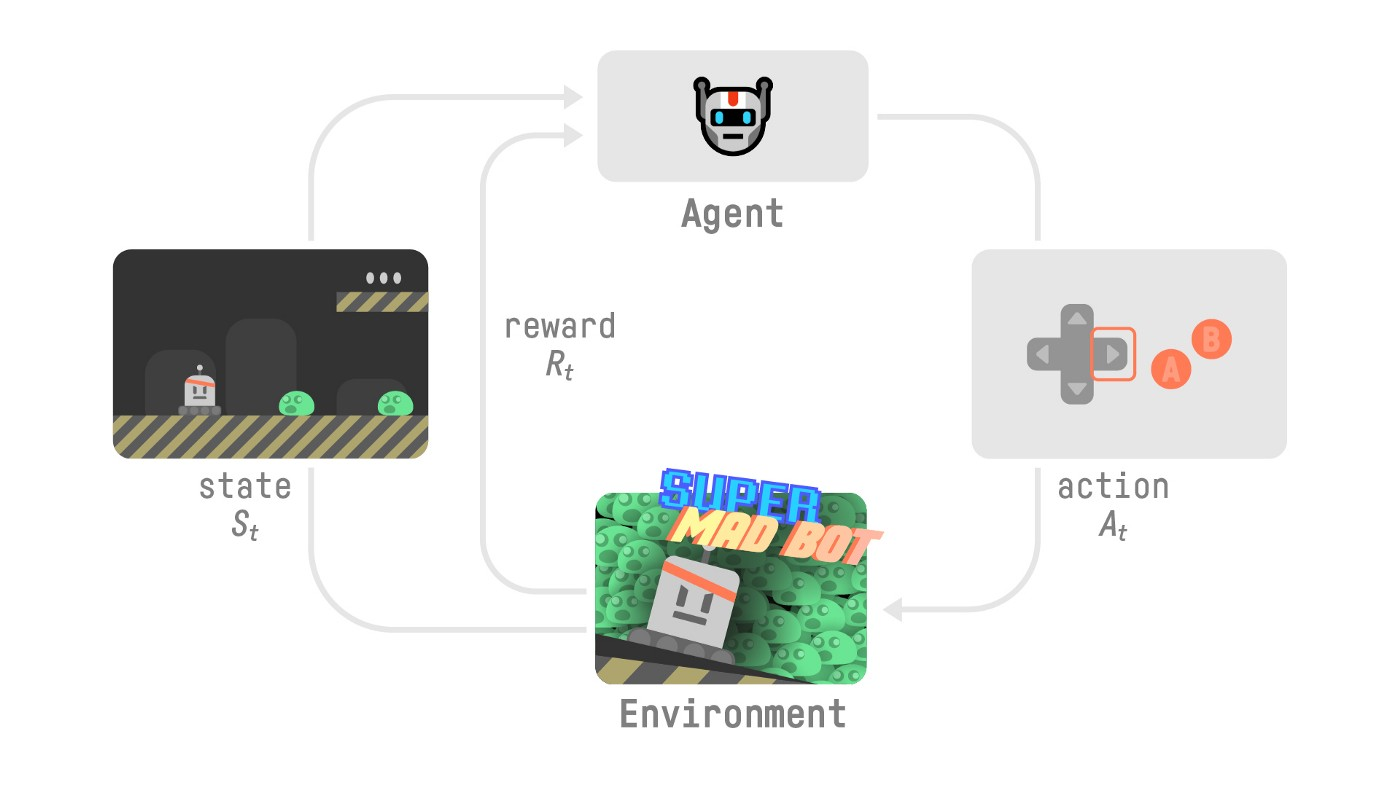
\includegraphics[width=0.6\linewidth,keepaspectratio]{rl108}
\end{center}

\end{frame}

%%%%%%%%%%%%%%%%%%%%%%%%%%%%%%%%%%%%%%%%%%%%%%%%%%%%%%%%%%%%%%%%%%%%%%%%%%%%%%%%%%
\begin{frame}[fragile]\frametitle{Generic Steps}

With Gym:

\begin{itemize}
\item We create our environment using \lstinline|gym.make()|
\item We reset the environment to its initial state with observation = env.reset()
\item At each step:

	\begin{itemize}
	\item Get an action using our model (in our example we take a random action)
	\item Using \lstinline|env.step(action)|, we perform this action in the environment and get

		\begin{itemize}
		\item obsevation: The new state (st+1)
		\item reward: The reward we get after executing the action
		\item done: Indicates if the episode terminated
		\item info: A dictionary that provides additional information (depends on the environment).
		\end{itemize}

	\item If the episode is done: We reset the environment to its initial state with \lstinline|observation = env.reset()|
	\end{itemize}
\end{itemize}

\end{frame}

%%%%%%%%%%%%%%%%%%%%%%%%%%%%%%%%%%%%%%%%%%%%%%%%%%%%%%%%%%%%%%%%%%%%%%%%%%%%%%%%%%
\begin{frame}[fragile]\frametitle{Generic Code}

With Gym:

\begin{lstlisting}
import gym

# First, we create our environment called LunarLander-v2
env = gym.make("LunarLander-v2")

# Then we reset this environment
observation = env.reset()

for _ in range(20):
  # Take a random action
  action = env.action_space.sample()
  print("Action taken:", action)

  # Do this action in the environment and get
  # next_state, reward, done and info
  observation, reward, done, info = env.step(action)
  
  # If the game is done (in our case we land, crashed or timeout)
  if done:
      # Reset the environment
      print("Environment is reset")
      observation = env.reset()
\end{lstlisting}

\end{frame}



%%%%%%%%%%%%%%%%%%%%%%%%%%%%%%%%%%%%%%%%%%%%%%%%%%%%%%%%%%%%%%%%%%%%%%%%%%%%%%%%%%
\begin{frame}[fragile]\frametitle{}
\begin{center}
{\Large Example: CartPole}
\end{center}
\end{frame}

%%%%%%%%%%%%%%%%%%%%%%%%%%%%%%%%%%%%%%%%%%%%%%%%%%%%%%%%%%%%%%%%%%%%%%%%%%%%%%%%%%
\begin{frame}[fragile]\frametitle{CartPole}

\begin{itemize}
\item Learn how to move the cart in the CartPole environment to maximize the duration (max 10s) the pole stays upright
\item Environment: Cart and Pole
\item Action: Move cart
\item Reward: Duration
\end{itemize}

\begin{lstlisting}
import gym
env = gym.make("CartPole-v1")
env.reset() # to initial state, starts simulation
env.render() # shows graphical view, cant close by cross click
env.close() # force close
\end{lstlisting}

\end{frame}

%%%%%%%%%%%%%%%%%%%%%%%%%%%%%%%%%%%%%%%%%%%%%%%%%%%%%%%%%%%%%%%%%%%%%%%%%%%%%%%%%%
\begin{frame}[fragile]\frametitle{Exercise}


\begin{lstlisting}
# Import gym in this cell

# Create the BipedalWalker-v3 environment and store it in a variable called env

# Reset the simulation to its initial state (this will start the simulation)

# Visualize the initial state
\end{lstlisting}

\end{frame}

%%%%%%%%%%%%%%%%%%%%%%%%%%%%%%%%%%%%%%%%%%%%%%%%%%%%%%%%%%%%%%%%%%%%%%%%%%%%%%%%%%
\begin{frame}[fragile]\frametitle{CartPole}

\begin{itemize}
\item Reset returns initial state, called Observations, 4 elements

\begin{center}
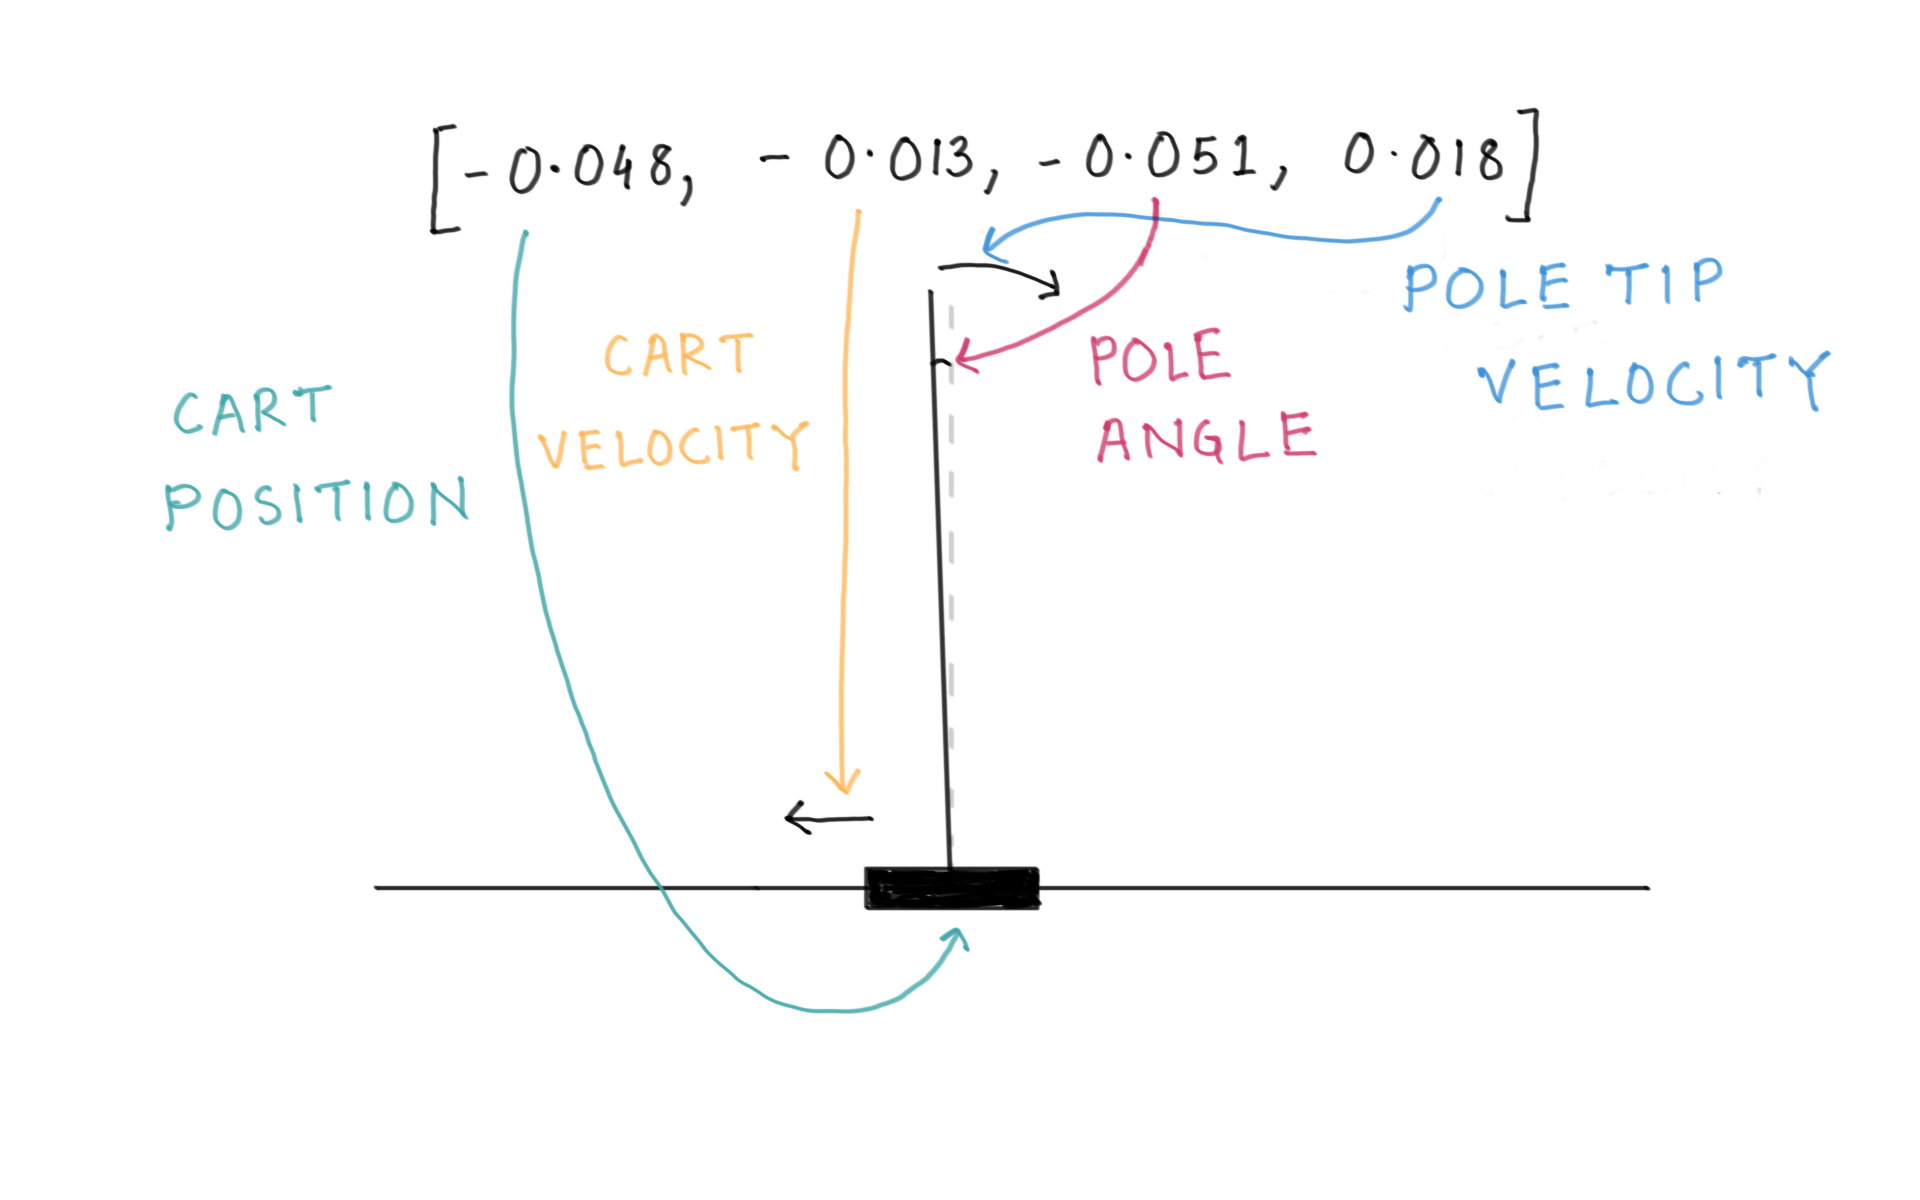
\includegraphics[width=0.5\linewidth,keepaspectratio]{rl60}
{\tiny (Ref: Fast RL course - Dibya Chakraborty)}
\end{center}

\item Are Observations continuous or discrete, scalar/vector/tensor, data-type?
\item `Box` for continuous, `(4,)` for 4 dimensional vector, lower range is first element in array, higher is the 2nd element. Data type is np.float32
\end{itemize}

\begin{lstlisting}
obs = env.reset() 
print(env.observation_space)

Box([-4.8000002e+00 -3.4028235e+38 -4.1887903e-01 -3.4028235e+38], [4.8000002e+00 3.4028235e+38 4.1887903e-01 3.4028235e+38], (4,), float32)
\end{lstlisting}


\end{frame}

%%%%%%%%%%%%%%%%%%%%%%%%%%%%%%%%%%%%%%%%%%%%%%%%%%%%%%%%%%%%%%%%%%%%%%%%%%%%%%%%%%
\begin{frame}[fragile]\frametitle{CartPole}

\begin{itemize}
\item Action is taken every 0.025 sec, to move right or left.
\item After reset, Env waits to receive action from Agent.
\item Here, actions are Discrete(2): 0,1, they are left and right.
\item Sending action is done by `step` with action in it.
\item Env will then simulate the change, and return the next observation.
\end{itemize}

\begin{center}
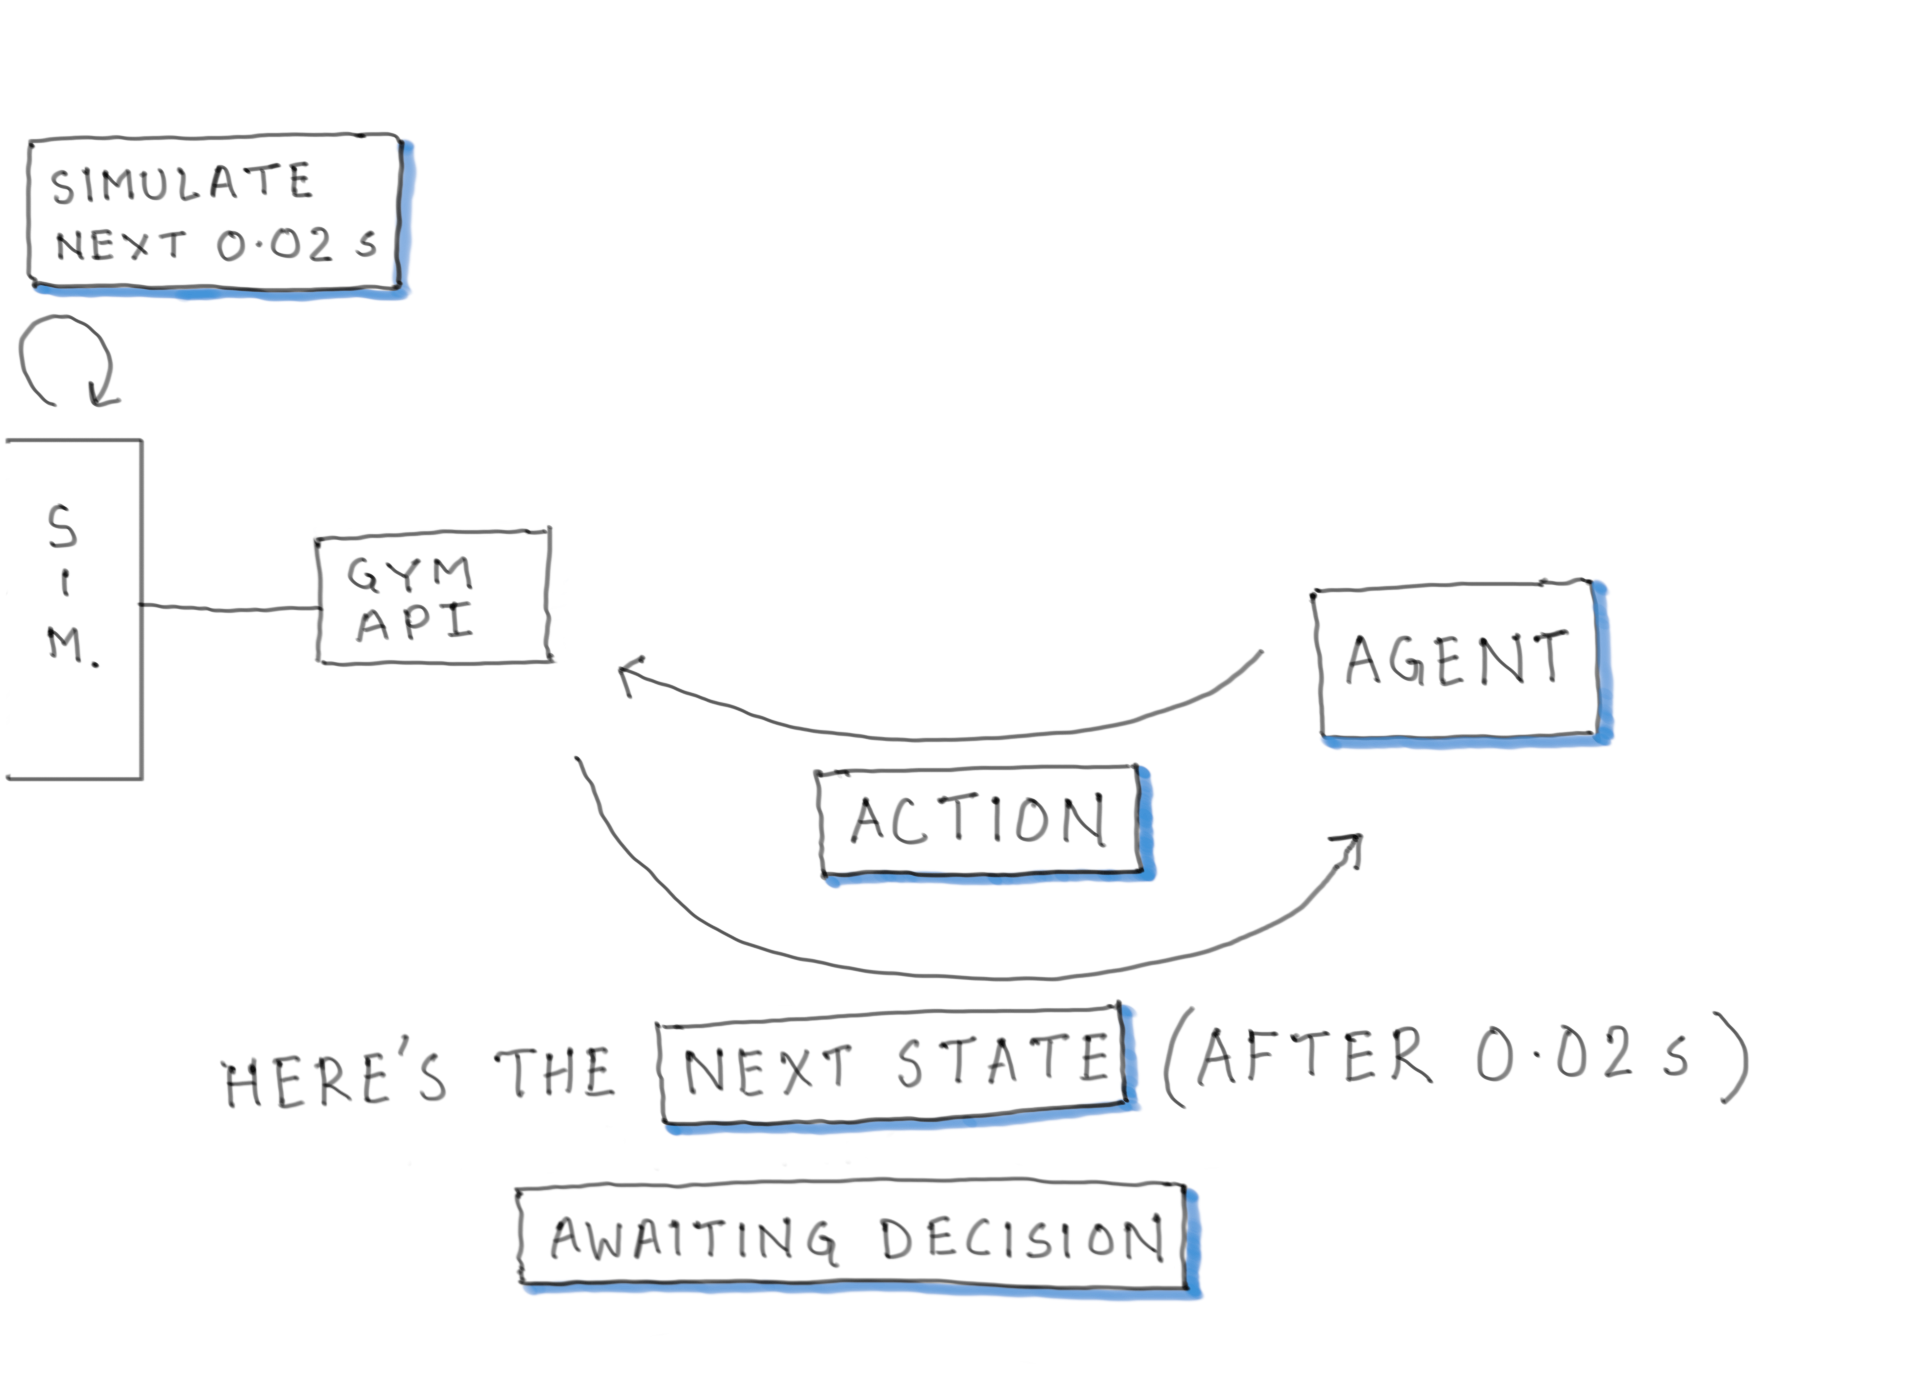
\includegraphics[width=0.3\linewidth,keepaspectratio]{rl61}
{\tiny (Ref: Fast RL course - Dibya Chakraborty)}
\end{center}

\begin{lstlisting}
new_obs, _, _, _ = env.step(0) # left
[ 0.03689718 -0.15012246  0.00797674  0.31285113]
new_obs, _, _, _ =  env.step(1) # right
[-0.02508183, -0.22606609,  0.0646681 ,  0.3370987 ]
\end{lstlisting}


\end{frame}

%%%%%%%%%%%%%%%%%%%%%%%%%%%%%%%%%%%%%%%%%%%%%%%%%%%%%%%%%%%%%%%%%%%%%%%%%%%%%%%%%%
\begin{frame}[fragile]\frametitle{CartPole}

Taking many actions in a loop

\begin{itemize}
\item reset() the env
\item take action 0 in a loop (push cart to the left)
\item call render() after every step
\item render shows that the cart is moved to left
\end{itemize}

\begin{lstlisting}
obs = env.reset()
for _ in range(30):
    print(obs)
    obs, _, _, _ = env.step(0)
    env.render()
\end{lstlisting}


\end{frame}

%%%%%%%%%%%%%%%%%%%%%%%%%%%%%%%%%%%%%%%%%%%%%%%%%%%%%%%%%%%%%%%%%%%%%%%%%%%%%%%%%%
\begin{frame}[fragile]\frametitle{CartPole}

Gym has a Reward function for CartPole
\begin{itemize}
\item If the pole is within +-12 degrees from vertical, reward is +1, else 0
\item Pole must  stay between environment bounds +- 2.4
\item Maximizing the cumulative reward is equivalent to maximizing the number of steps the pole stays upright.
\item $duration=0.02s \times num steps$
\item Maximizing the cumulative reward is equivalent to maximizing the duration the pole stays upright.
\end{itemize}

\begin{lstlisting}
obs = env.reset()
for _ in range(30):
    print(f"Pole angle at step start: {np.degrees(obs[2])}", end=" ")
    obs, reward, _, _  = env.step(0)
    print(f"Reward in this step: {reward}")
Pole angle at step start: -1.9815118943994086 Reward in this step: 1.0
Pole angle at step start: -1.9753829089133865 Reward in this step: 1.0
:		
\end{lstlisting}


\end{frame}

%%%%%%%%%%%%%%%%%%%%%%%%%%%%%%%%%%%%%%%%%%%%%%%%%%%%%%%%%%%%%%%%%%%%%%%%%%%%%%%%%%
\begin{frame}[fragile]\frametitle{CartPole}

\begin{itemize}
\item Episodes decide till what duration the rewards need to be accumulated.
\item In games, the episodes end at Win/Loss/Terminal states.
\item The third element of the return value of env.step(action) indicates if we have reached a terminal state
\item In Cartpole, there is no reward 0, but thats the Terminal state (pole down, boundary touch). Pole is upright and 500 steps are reached, then we win.
\end{itemize}

\begin{lstlisting}
obs = env.reset()
for _ in range(30):
    print(f"Pole angle at step start: {np.degrees(obs[2])}", end=" ")
    obs, reward, done, _  = env.step(0)
    print(f"Pole angle at step end: {np.degrees(obs[2])}", end=" ")
    print(f"Reward in step: {reward}, done: {done}")
		
Pole angle at step start: 2.5225715240513926 Pole angle at step end: 2.5628541577896797 Reward in step: 1.0, done: False
Pole angle at step start: 2.5628541577896797 Pole angle at step end: 2.9540647813957777 Reward in step: 1.0, done: False
Pole angle at step start: 2.9540647813957777 Pole angle at step end: 3.6964366026209015 Reward in step: 1.0, done: False
:		
\end{lstlisting}


\end{frame}

%%%%%%%%%%%%%%%%%%%%%%%%%%%%%%%%%%%%%%%%%%%%%%%%%%%%%%%%%%%%%%%%%%%%%%%%%%%%%%%%%%
\begin{frame}[fragile]\frametitle{CartPole}

Doing multiple episodes
\begin{itemize}
\item Once done is True, we should not take any more actions
\item To collect, call env.reset() if you want to restart the simulation
\end{itemize}

\begin{lstlisting}
for ep in range(5):
    print(f"Episode number is {ep+1}")
    obs = env.reset()
    while True:
        print(f"Pole angle at step start: {np.degrees(obs[2])}", end=" ")
        obs, reward, done, _  = env.step(0)
        print(f"Pole angle at step end: {np.degrees(obs[2])}", end=" ")
        print(f"Reward in step: {reward}, done: {done}")
        if done:
            break
						
Episode number is 1
Pole angle at step start: 1.1183983506183337 Pole angle at step end: 1.1099812877349993 Reward in step: 1.0, done: False
:
Episode number is 2
Pole angle at step start: 0.515380400430025 Pole angle at step end: 0.5154796938477244 Reward in step: 1.0, done: False
:
\end{lstlisting}

\end{frame}

%%%%%%%%%%%%%%%%%%%%%%%%%%%%%%%%%%%%%%%%%%%%%%%%%%%%%%%%%%%%%%%%%%%%%%%%%%%%%%%%%%
\begin{frame}[fragile]\frametitle{}
\begin{center}
{\Large Example: Lunar Lander}
\end{center}

{\tiny (Ref: Deep RL Class Hugging Face Unit 1: Train your first Deep Reinforcement Learning Agent)}

\end{frame}

%%%%%%%%%%%%%%%%%%%%%%%%%%%%%%%%%%%%%%%%%%%%%%%%%%%%%%%%%%%%%%%%%%%%%%%%%%%%%%%%%%
\begin{frame}[fragile]\frametitle{Introduction}

\begin{itemize}
\item Objective:  train our agent, a Lunar Lander, to land correctly on the moon. 
\item To do that, the agent needs to learn to adapt its speed and position(horizontal, vertical, and angular) to land correctly.
\end{itemize}

\begin{center}
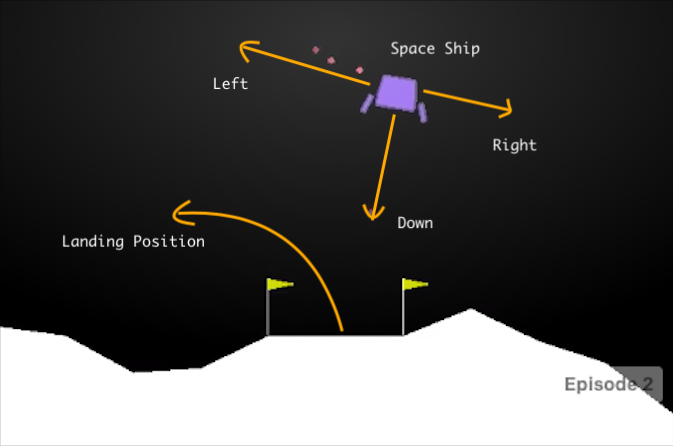
\includegraphics[width=0.5\linewidth,keepaspectratio]{rl109}

{\tiny (Ref: Train Your Lunar-Lander | Reinforcement Learning | OpenAIGYM | by Shiva Verma | Medium)}

\end{center}



\end{frame}

%%%%%%%%%%%%%%%%%%%%%%%%%%%%%%%%%%%%%%%%%%%%%%%%%%%%%%%%%%%%%%%%%%%%%%%%%%%%%%%%%%
\begin{frame}[fragile]\frametitle{Observation Space}

We see with Observation Space Shape (8,) that the observation is a vector of size 8, where each value contains different information about the lander:

\begin{itemize}
\item Horizontal pad coordinate (x)
\item Vertical pad coordinate (y)
\item Horizontal speed (x)
\item Vertical speed (y)
\item Angle
\item Angular speed
\item If the left leg has contact point touched the land
\item If the right leg has contact point touched the land
\end{itemize}

\begin{lstlisting}
# We create our environment with gym.make("<name_of_the_environment>")
env = gym.make("LunarLander-v2")
env.reset()
print("_____OBSERVATION SPACE_____ \n")
print("Observation Space Shape", env.observation_space.shape)
print("Sample observation", env.observation_space.sample()) # Get a random observation
\end{lstlisting}

\end{frame}

%%%%%%%%%%%%%%%%%%%%%%%%%%%%%%%%%%%%%%%%%%%%%%%%%%%%%%%%%%%%%%%%%%%%%%%%%%%%%%%%%%
\begin{frame}[fragile]\frametitle{Action Space}

The action space (the set of possible actions the agent can take) is discrete with 4 actions available:

\begin{itemize}
\item Do nothing,
\item Fire left orientation engine,
\item Fire the main engine,
\item Fire right orientation engine.
\end{itemize}

\begin{lstlisting}
print("\n _____ACTION SPACE_____ \n")
print("Action Space Shape", env.action_space.n)
print("Action Space Sample", env.action_space.sample()) # Take a random action
\end{lstlisting}

\end{frame}

%%%%%%%%%%%%%%%%%%%%%%%%%%%%%%%%%%%%%%%%%%%%%%%%%%%%%%%%%%%%%%%%%%%%%%%%%%%%%%%%%%
\begin{frame}[fragile]\frametitle{Reward Function}

The function that will gives a reward at each timestep:

\begin{itemize}
\item Moving from the top of the screen to the landing pad and zero speed is about 100~140 points.
\item Firing main engine is -0.3 each frame
\item Each leg ground contact is +10 points
\item Episode finishes if the lander crashes (additional - 100 points) or come to rest (+100 points)
\end{itemize}

We may want to create a vectorized environment (method for stacking multiple independent environments into a single environment) of 16 environments, this way, we'll have more diverse experiences during the training.

\begin{lstlisting}
# Create the environment
env = make_vec_env('LunarLander-v2', n_envs=16)
\end{lstlisting}

\end{frame}

%%%%%%%%%%%%%%%%%%%%%%%%%%%%%%%%%%%%%%%%%%%%%%%%%%%%%%%%%%%%%%%%%%%%%%%%%%%%%%%%%%
\begin{frame}[fragile]\frametitle{Solve the RL problem}

Meaning, Create the Model.
 
\begin{itemize}
\item Using Stable Baselines3 (SB3).
\item SB3 is a set of reliable implementations of reinforcement learning algorithms in PyTorch.
\item Going to use SB3 PPO. PPO (aka Proximal Policy Optimization) is one of the of the SOTA (state of the art) Deep Reinforcement Learning algorithms
\item PPO is a combination of:
	\begin{itemize}
	\item Value-based reinforcement learning method: learning an action-value function that will tell us what's the most valuable action to take given a state and action.
	\item Policy-based reinforcement learning method: learning a policy that will gives us a probability distribution over actions.
	\end{itemize}

\end{itemize}

\end{frame}

%%%%%%%%%%%%%%%%%%%%%%%%%%%%%%%%%%%%%%%%%%%%%%%%%%%%%%%%%%%%%%%%%%%%%%%%%%%%%%%%%%
\begin{frame}[fragile]\frametitle{SB3 setup}

\begin{itemize}
\item Create environment (done above)
\item Define the model \lstinline|model = PPO("MlpPolicy")|
\item Train the agent with \lstinline|model.learn| and define the number of training timesteps
\item Save
\end{itemize}


\begin{lstlisting}
# Create environment
env = gym.make('LunarLander-v2')

# Instantiate the agent
model = PPO('MlpPolicy', env, verbose=1)
# Train the agent
model.learn(total_timesteps=int(2e5))
# Save the model
model_name = "ppo-LunarLander-v2"
model.save(model_name)
\end{lstlisting}

\end{frame}

%%%%%%%%%%%%%%%%%%%%%%%%%%%%%%%%%%%%%%%%%%%%%%%%%%%%%%%%%%%%%%%%%%%%%%%%%%%%%%%%%%
\begin{frame}[fragile]\frametitle{Evaluate}

\begin{itemize}
\item When you evaluate your agent, you should not use your training environment but create an evaluation environment.
\item Mean reward got is 204.16 +/- 38.25 after training for 1 million steps, which means that our lunar lander agent is ready to land on the moon 
\item By using \lstinline|package_to_hub| you evaluate, record a replay, generate a model card of your agent and push it to the hub.
\end{itemize}

\begin{lstlisting}
# Create a new environment for evaluation
eval_env = gym.make("LunarLander-v2")

# Evaluate the model with 10 evaluation episodes and deterministic=True
mean_reward, std_reward = evaluate_policy(model, eval_env, n_eval_episodes=10, deterministic=True)

# Print the results
print(f"mean_reward={mean_reward:.2f} +/- {std_reward}")
\end{lstlisting}


\end{frame}



